\chapter{Text Analysis}\label{chapter:analysis}

\section{Introduction}
In this chapter, the social network posts text analyses originally featured in Socneto are described. 

The solved problems are presented in the section \ref{sec:posibilities} of this chapter. First, the motivation behind the choice of these problems and other possible types of analyses is discussed. Furthermore, a comparison of different input data types and their limitations is given. 
In the sections \ref{sec:topic_modelling} and \ref{sec:sentiment}, the chosen problems are described precisely together with selected solutions. A quick comparison of possible methods, the theory behind them and implementation details are provided for each problem.

Section \ref{sec:experiments} of this chapter is dedicated to a discussion of results and a conclusion.

\section{Natural Language Processing - Possibilities and Drawbacks}
\label{sec:posibilities}

As main goal of Socneto is analysis of posts from social networks, this section provides an introduction to a natural language processing (NLP). In Deep Learning book \cite{DeeplearningBook}, NLP is defined as \textit{"...the use of human languages, such as English or French, by a computer."}.

\subsection{What Is Possible}

The main intention of Socneto is to present automatically analysed data from various social networks. Socneto is extensible in many directions including new social networks and new types of analyses, but some analysis types are provided by default. Chapter \ref{chapter:implementation} of this documentation describe how to choose, obtain and store data from Reddit and Twitter. The question is, what to do with them. \par
NLP offers a variety of problems to solve. Some of them are  beyond our focus, for instance, conversion between written and oral language. We could imagine using this to analyse short videos published on Twitter. This could give us more text for analyses, but we  focus first on  basic analysis of the text we have.\par Another possible way of natural language processing is \textbf{syntax analysis} - examination of the formal structure of words, sentences and larger parts of the text. \textit{Sentence breaking} or \textit{word segmentation}, which divides the text into smaller, further analysed parts are included in the pipeline for text preprocessing. The task of \textit{lemmatization}, also used in preprocessing, lies in finding a base form of a given words, meaning for example nominative of singular for nouns or infinitive for verbs. The analysis can then continue with \textit{morphological segmentation}, which divides words into smaller parts, morphemes. To return to whole sentences, different types of trees are used to represent the structure of sentences and dependencies within a sentence (see Figure \ref{fig:trees}).
\begin{figure}[h]
\centering
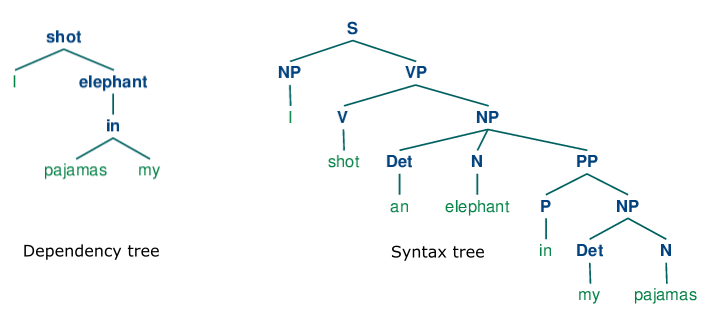
\includegraphics[width=1\textwidth]{diagrams/syntax_depedency_trees.png}
\caption{
An example of the syntax and dependency tree. Dependency tree, as the name indicates, describes dependencies between words. Such dependencies are of various types, for example an elephant in the example is an direct object of the shooting action. A root of such tree is typically a predicate of the sentence. On the other hand, syntax tree represents syntactic structure of the sentence according to the grammar. The root of the tree is \textit{sentence}, which is split to noun and verb phrase. These can be further divided into phrases compound from particular instances of parts of speech (e.g. nouns, adverbs, verbs, prepositions etc).
\newline \textit{Source: \cite{NLTKbook}}}
\label{fig:trees}
\end{figure}\par All previously mentioned treatments and many others are available for syntax analysis and most of them are needed for whatever task is performed, but they do not provide much information about the meaning of the text, at least for a human reader. \par More suitable for this purpose is the part of NLP dedicated to \textbf{semantic analysis}. Again, it contains various methods from natural language text generation to  recognition of homonymy or polysemy of given words. It could solve sophisticated assignments as answering questions about the input text document or  translation. Another possible task is to find in the text so-called named entities - like persons, months or cites - or linking these entities to some knowledge base. We can try to recognize the formality of the text, its sentiment, main topics or even try to automatically modify the text to be clearer. \par It is not necessary to be limited to text analysis only. In addition to speech recognition, it is also possible to engage in computer vision for extracting information from pictures. The importance of social networks data does not lie only in user contribution, but also in the metadata. Interesting results can be obtained via study of different user groups, their relationships to other groups, or different topics and opinions together with some demographic data.

\subsection{The Nature of the Data}
 Social networks have become important communication medium in recent times. They have the power to influence many people whether it is shopping, politics, environmental responsibility or the newest trends. So there are many reasons for understanding them. Data stored in networks are growing every second and it is not in human power to consume all of them. The problem of obtaining this data is solved by the acquiring mechanism of our platform as described in other sections of the documentation (chapter \ref{chapter:implementation}).
 \par
 Inputs to natural language processing can be data of many kinds. Both syntactic and semantic models can be trained on \textit{treebanks}. An example of a treebank is in Figure \ref{fig:pdt}). A treebank is a parsed corpus with various types of annotations.
For machine translation documents with many language versions are appropriate.

\begin{figure}
\centering
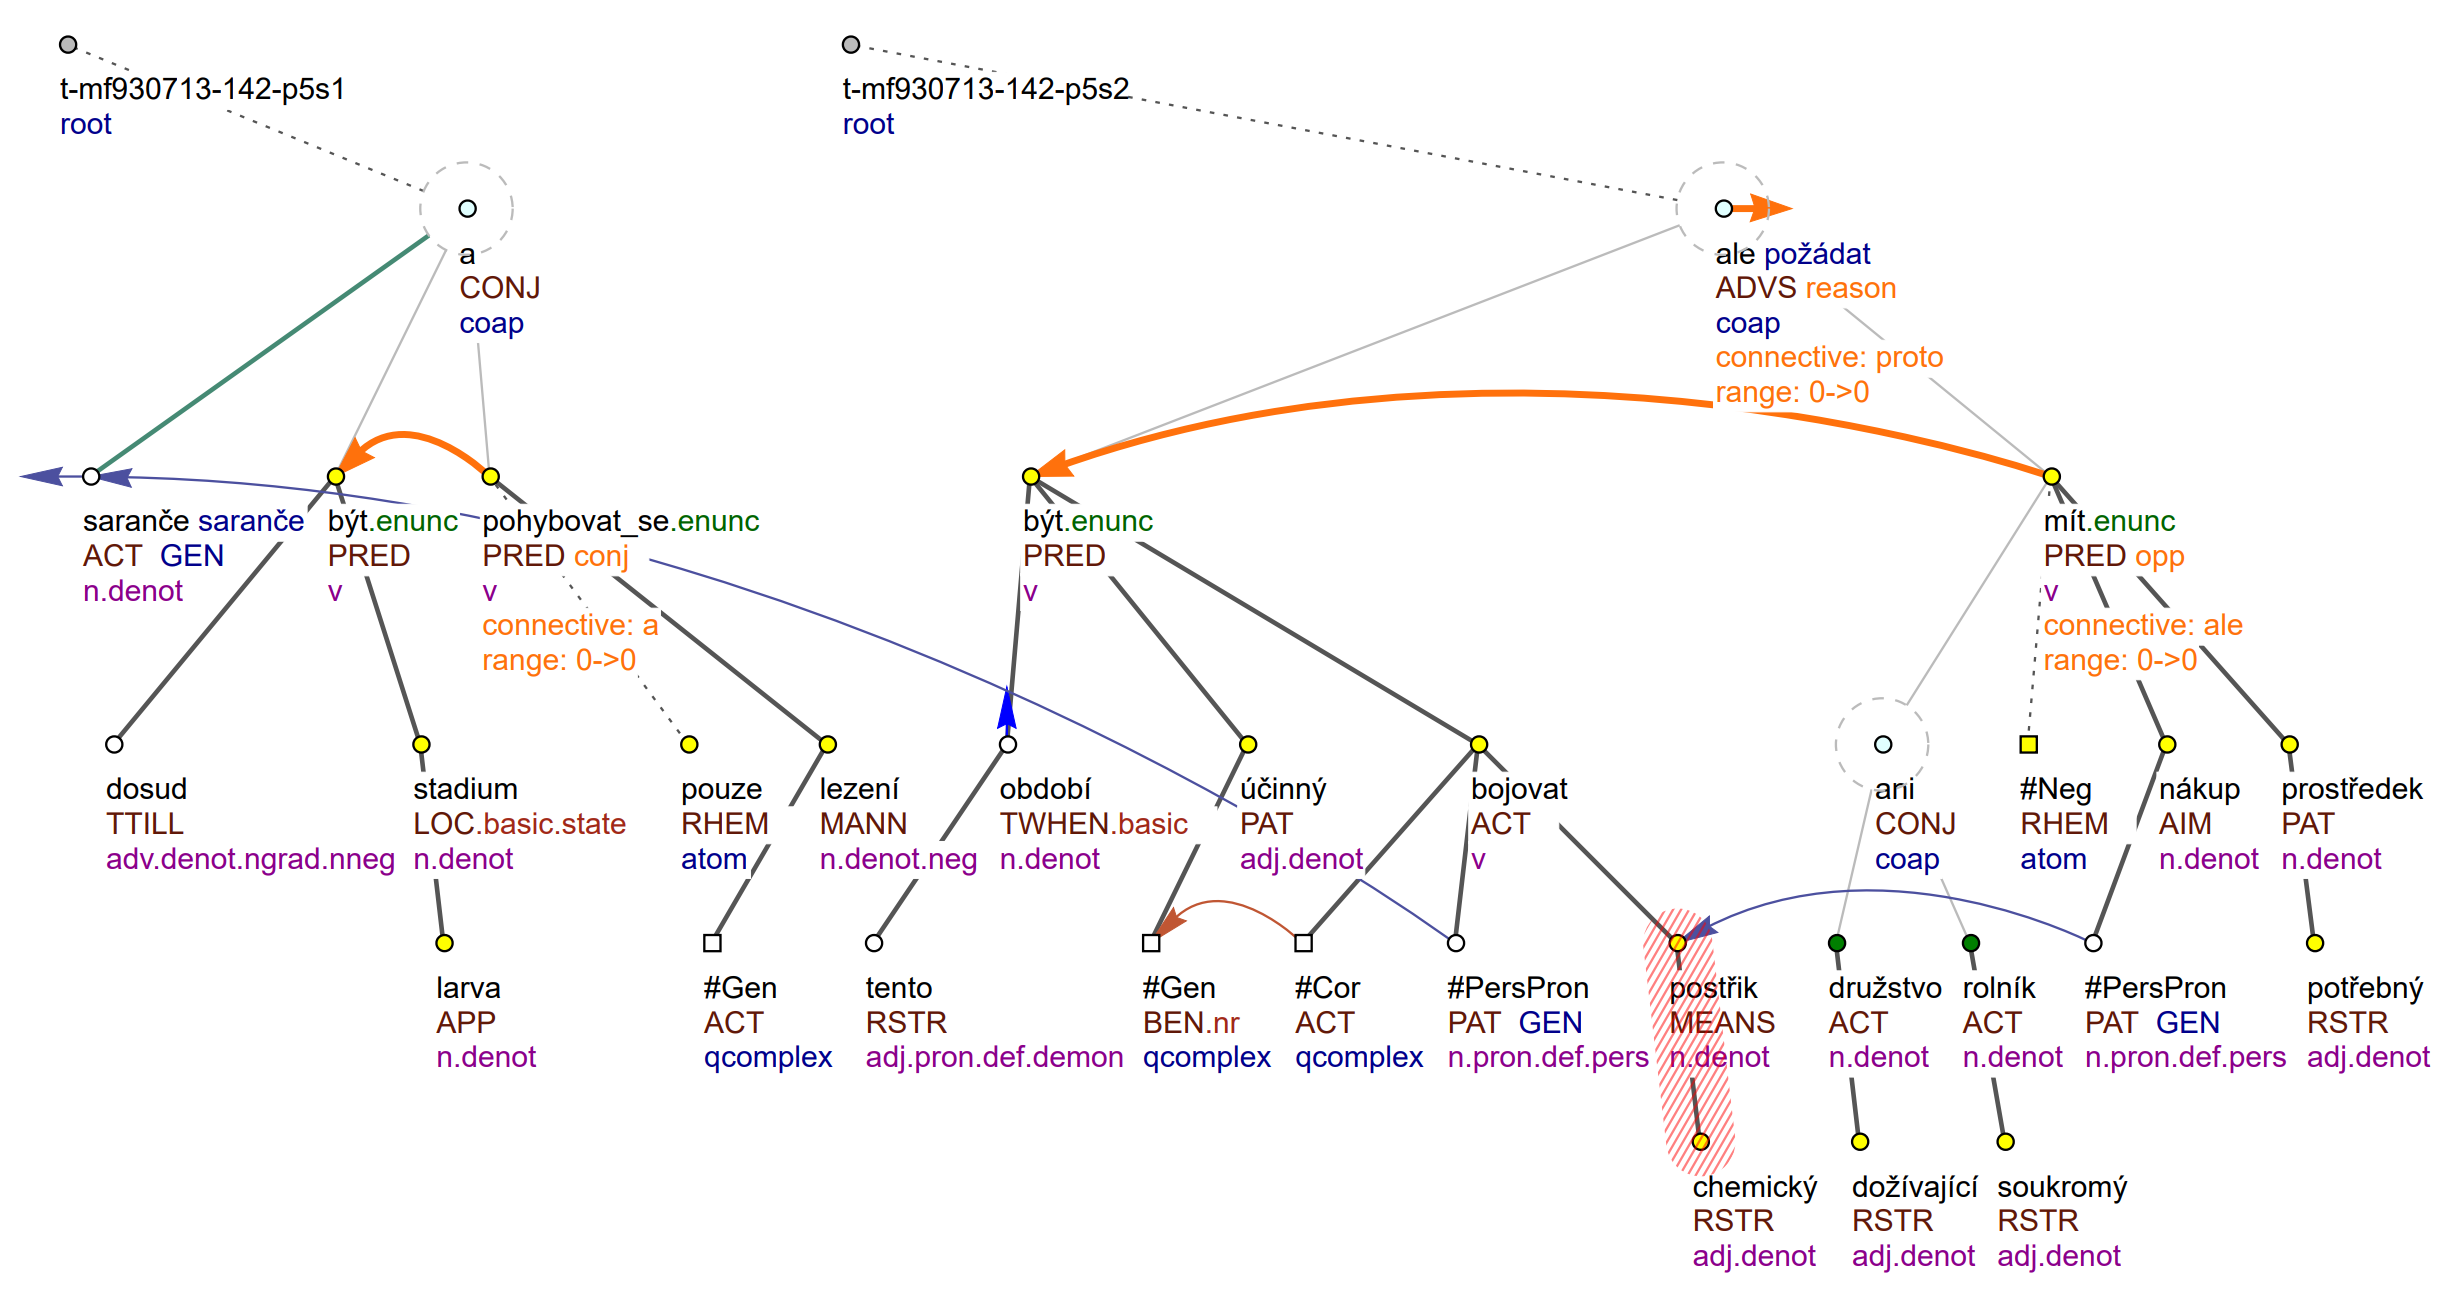
\includegraphics[width=1\textwidth]{diagrams/prague_dep_treebank.png}
\caption{
Prague dependency treebank example~\cite{PDT35} for the sentences: \textit{Sarančata jsou doposud ve stadiu larev a pohybují se pouze lezením. V tomto období je účinné bojovat proti nim chemickými postřiky, ale dožívající družstva ani soukromí rolníci nemají na jejich nákup potřebné prostředky}. This treebank contains dependency trees, but is is just one of many possibilities. This example is from Prague dependency treebank, which offers different layers of annotations. Red strips over words \textit{chemický} and \textit{postřik} marks multiword phrase, conjunction between \textit{rolník} and \textit{družstvo} is expressed as by one type of nodes, blue lines denotes coreference etc.}
\label{fig:pdt}
\end{figure}

Eurotra \cite{diane1995final} is, for example, almost twenty years lasting project of the European Commission dedicated to machine translation started on the latest seventieths. EU administrative documents in French and English served as datasets. \par
Topic modeling is typically applied on a big set of medium length documents (e.g.  scientific articles). In contrast, data from tweets and Reddit are different. Tweets are short snippets of text full of odd characters, newlines, and ends of lines. They contain pictures, emoji, a mixture of different languages, slang expressions, and grammatical errors. And they are very short, sometimes only one sentence long, few hashtags and a link or a picture.
Texts from Reddit are larger, but there is a challenging aspect of both social sites. The data has tree structure: Tweet and retweets or comments in the case of Twitter and main thread post with replies in the case of Reddit. These replies or comments can be even shorter than their parent post and/or do not mention previously said things explicitly. For performing a reasonable work of analysis it is necessary to have all these pieces of information together. \par Questions about the meaning of the text have another difficulty, which is, however, part of their attraction. They do not have always an unambiguous response. In the case of topic modeling, the goal is to identify general topics of a given text. These topics are not necessarily mentioned explicitly in the text and are then obviously hard to agree on them, especially if there is no given set of topics to choose from. Semantic analysis is a little bit easier. Evaluation of extremely positive or negative texts is mostly consistent among people. But of course, there is text somewhere in between, where classification is not so simple. Sentiment analysis must also deal with things like sarcasm or irony. It is not so complicated to learn a model when positive words like ``good'', ``nice'', ``favorite'' or ``love'' means positive sentiment of the classified text, but it is much harder to distinguish situations, where they mean the opposite.

The second problem connected with data quantity is a human inability to read them all. For this purpose, out-of-the-box analysis is aggregated to get a better overview. \par
\subsection{Choices for Socneto}
For these reasons we decided to focus on semantic types of analysis of data and to present two types of semantic analysis - \textit{sentiment analysis} and \textit{topic modeling}. Both these analyses helps us with extracting a meaning and their results can be aggregated in a reasonable way. Topic modeling allows us to identify popular topics themselves or to find other often related topics to the given one. So we can find out, what are people on social sites talking about. The second provided analysis - \textit{sentiment analysis} gives us an overview of their opinion about those topics. Both types of analysis are applied to a big bunch of data and return summary analysis, which is another useful feature. There are typically too many user posts to analyse, so inspecting each of them separately would produce an overwhelming amount of information and this does not solve the need for automatic analysis. 

\subsection{Machine Learning}

As in almost every machine learning application, possible methods can be supervised or unsupervised. Supervised methods require a dataset (sometimes called gold data), where  examples are problem instances together with correct answers. The learning algorithm then tries to find patterns or rules for classification and (iteratively) compares its answers with the correct ones. On the contrary, we need no correct answers for unsupervised learning. It is typically based on searching in the space of parameters to minimize some function (\textit{loss function)}. And it is also possible to solve tasks without machine learning at all by creating a set of hand-made rules. This approach is historically the first, but certainly not in the results.
\section{Topic Modeling (TM)}
\label{sec:topic_modelling}
Topic modeling task can be described by one of the following definitions:
\par
\begin{enumerate}

  \item A classification of a bunch of documents into a given number of topics together with learning typical keywords for each topic.
  \begin{itemize}
      \item \textbf{Input:} A set of documents, desired number of topics (integer, greater than zero).
      \item \textbf{Output:} Estimated probability distribution of topics for each document, estimated probability distribution of words for each topic.
    \end{itemize}
  \item Finding a list of words (=topics) associated with given data and their importance or distribution (which is what Socneto wants to do). 
  \begin{itemize}
      \item \textbf{Input:} Text for analysis (all tweets or posts together.)
      \item \textbf{Output:} A set of words best representing input.
    \end{itemize}

As there exists solution for the problem A, there also exists solution for problem B. It is true, because problem B can be transferred to the problem A by setting a count of topics to 1 and searching only for keywords. This does not solve the problem of finding abstraction topics not mentioned in the text but gives a quite good overview of the input data.
  \item A classification of texts into given topics.
   \begin{itemize}
      \item \textbf{Input:} Texts for classification, topics to choose from
      \item \textbf{Output:} One label from given topics for each text.
    \end{itemize}

\end{enumerate}
\subsection{Methods}
Regarding supervised methods, it is possible to use any known supervised classification algorithm. Among others support vector machines, logistic regression or neural networks belong here. The intended usage of Socneto is an application on data from many different areas, so we cannot define topics in advance, which is the reason, why our problem is not following definition C. \par This determines us to use unsupervised methods. For TM defined as in definition A, two mainly used methods are Latent Semantic Analysis (LSA) \cite{LSA} and Latent Dirichlet Allocation (LDA) \cite{LDA}. They are both based on the same assumptions, but LDA is an improved version of LSA with better performance. Topic modeling as in definition B was chosen for implementation, so we use LDA for it. A detailed description of theory and implementation is available in the following section. \par
Because LDA used in the described way (i.e. following the definition B) can find only words explicitly expressed in the text, we wanted to enrich the analysis by some more abstract topics. It can be done via solving \textit{entity linking} problem, which assigns hierarchical structure of categories to found entities/topics. The structure for classification is called the knowledge base and can be extracted automatically for example from Wikipedia. Or we can solve another problem - \textit{Named Entity Recognition} (NER). Algorithms for NER are able to tag each named entity by its category. Categories vary depending on implementation and training data, but categories like city, proper name, date, language or month can occur. This is supervised learning, but with a limited quantity of target classes and allows us to search for topics in specific categories provided by NER.
\par

\subsection{NER}
The task of finding named entities in the text and classifying them into the right category.
   \begin{itemize}
      \item \textbf{Input:} Unstructured text (= natural language), categories
      \item \textbf{Output:} Classification into right category if exists for all words (see Figure \ref{fig:NER})
    \end{itemize}
    
NER can be divided into two subtasks - identification of entities and their classification. As for every classification task, we can use supervised machine learning or rule-based system written by an expert. Another useful feature of this analysis is to recognize not only words but whole phrases (e.g.  National Park). This analysis can served as another tool for exploring the data. It allows filtering topics by categories like \textit{person} or \textit{place}. It can also helps to improve topic searching, as named entities are typically important int the text and NER is able to find pronoun references to them. Without such references, the word can occur just for one time and could appear as unimportant to LDA.

\begin{figure}[h]
\centering
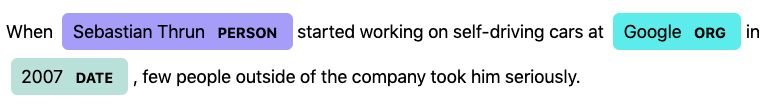
\includegraphics[width=1\textwidth]{diagrams/NER.png}
\caption{
An output of the Named Entity Recognition. Example from the SpaCy library documentation}
\label{fig:NER}
\end{figure}
Our analysis provides classification into 18 classes (see Table \ref{tab:nerclasses}) as we used third-party library SpaCy\footnote{\url{www.spacy.io}}, where these classes are predefined. 

\begin{table}[h]
\centering
\footnotesize
\begin{tabular}{ l p{0.7\textwidth} }
\hline
  \textbf{Class} & \textbf{Description} \\ \hline \hline
  PERSON & People, including fictional. \\ \hline
 NORP &  Nationalities or religious or political groups. \\ \hline
 FAC &  Buildings, airports, highways, bridges, etc. \\ \hline
 ORG &  Companies, agencies, institutions, etc.\\ \hline
 GPE &  Countries, cities, states.\\ \hline
 LOC &  Non-GPE locations, mountain ranges, bodies of water.\\ \hline
 PRODUCT &  Objects, vehicles, foods, etc. (Not services.)\\ \hline
 EVENT &  Named hurricanes, battles, wars, sports events, etc.\\ \hline
 WORK\_OF\_ART &  Titles of books, songs, etc.\\ \hline
 LAW &  Named documents made into laws.\\ \hline
 LANGUAGE &  Any named language.\\ \hline
 DATE &  Absolute or relative dates or periods.\\ \hline
 TIME &  Times smaller than a day.\\ \hline
 PERCENT &  Percentage, including "\%". \\ \hline
 MONEY &  Monetary values, including unit.\\ \hline
 QUANTITY &  Measurements, as of weight or distance.\\ \hline
 ORDINAL &  “first”, “second”, etc.\\ \hline
 CARDINAL &  Numerals that do not fall under another type.\\ \hline
 \end{tabular}
\caption{Classes in NER (spaCy)}
\label{tab:nerclasses}
\end{table}

 \par The used library, SpaCy, has pre-trained models for tagging and entity recognition for different languages. Algorithms in this library are not exactly based on one article, that could be named. Based on the GitHub discussion \cite{NERSpacy}, spaCy implementation of NER can be shortly described as classification using Convolutional Neural Networks (CNN) as in paper \cite{NERpaper}, but residual connections are used instead of dilatation and there are some other minor differences. Together with residual connections, there are two other important features - word embedding strategy using subword features and a transition-based approach. All three principles will be shortly described now. 
 \subsubsection{Word Embeddings with Subwords}
 Word embeddings are numbers or numerical vectors representing some categorical features. Their interesting feature is that when the source categories are near to each other, their embeddings are as well. Each dimension of the vector represents a different property of the word. One famous example for all: Embedding for the word 'Queen' can be almost exactly computed by the following formula on respective embeddings
 $king - man + woman$. A limitation of the original paper on embeddings \cite{mikolov2013efficient} concept was its inability to represent the morphological structure of the word. Embeddings were created based on the corpus and their occurrence in a similar context. It means, that no embedding exists for a newly seen word, even if it is morphologically very similar to a known one. Numeric representation of n-gram taken into account during the computation of an embedding is a solution to the problem.\cite{ngram_embedd}
 After this step, all words are represented by their embeddings and the following processing is performed only on them. 
 \subsubsection{CNN with Residual Connections}
 The convolutional neural network (see Chapter 9 in \cite{DeeplearningBook}) is a type of deep neural network with good ability to represent structures in the space. The input of this network is not a vector but a matrix (like a picture represented by values of its pixels). There is one single path from the input to the output of the network and every layer consists in the application of a filter or multiplication by a kernel on the sliding window.
 \par
In the case of residual connections, the network is split into smaller parts. To avoid  vanishing of information during the flow through the network, new shortcut connections (= residual connections) are added between some nodes. This approach is widely used in image recognition but also spread to other fields (see Figure \ref{fig:resnet}).
\begin{figure}[h]
\centering
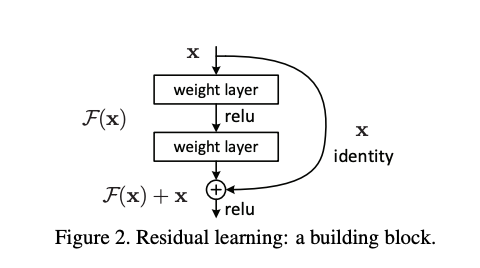
\includegraphics[width=0.7\textwidth]{diagrams/residual_connection.png}
\caption{
An example of the network for image recognition with residual connections. Residual network is a chain of layers with connections between as in deep forward networks, but there is also added connection marked as x identity, because in this case the activation function on the residual is identity function, which creates shortcut for strengthening information flow through the network.
\textit{source: \cite{DBLP}}}
\label{fig:resnet}
\end{figure}

\subsubsection{Transition Based Approach}
This approach consists of a sequence of small steps. In every step, only one word from the buffer is labeled or just one change to the configuration is applied \cite{daume2006practical}.

\subsection{LDA}
%co chceme, co je vstup a vystup, jak se to da udelat 
As mentioned above, Socneto uses LDA in the following manner:
   \begin{itemize}
      \item \textbf{Input:} A list of words (extracted from the text)
      \item \textbf{Output:} Top $n$ (in our case $n=10$, but it can be changed) words describing input.
    \end{itemize}
As the data are full of odd characters, newlines, and ends of lines, the first step is to clean the data. Our first trials have shown that adjectives are rarely useful, even indeed they make results messy and not informative at all. The same applies to pronouns, so words of both categories are removed. We can do this because the input of LDA is just a list of words, thus we can remove those words we don't want to be considered. We use the same pipeline described in the section \ref{sec:implementTM} because it helps us with the filtration. \par
%Now is time for the description of the theory. 
The previously mentioned LSA is an ancestor of LDA and it is better for showing basic ideas behind these two methods. LSA (same as LDA) is based on two assumptions: 
\begin{itemize}
  \item Every document contains a mixture of topics.
  \item Every topic is connected with different, but not necessarily disjoint, set of words. 
\end{itemize}
LSA than creates a matrix of documents contra terms, where values are \textit{tf\_idf}-s, where \textit{tf} stands for a term frequency
\[ tf = \frac{term\_occurences}{number\_of\_words\_in\_document} \]
and this is count over the whole corpus of documents (do not forget, that LSA is primarily applied on the corpus of different documents), while \textit{idf} is inverse document frequency
\[\frac{number\_of\_documents}{number\_of\_documents\_with\_term}.\]\textit{Idf} works as an evaluation of the importance of the word. The result is then: \[tf\_idf = tf \cdot idf .\] This matrix is then decomposed using \textit{singular value decomposition} (SVD). Decomposition gives us three matrices - $S$, $U$ and $V$. Matrix $S$ is always diagonal and each element on the diagonal represents one topic. Matrices $U$ and $V$ are document-topic and term-topic matrices respectively (see Figure \ref{fig:svd}) and they contains probability distributions. 

\begin{figure}[ht]
\centering
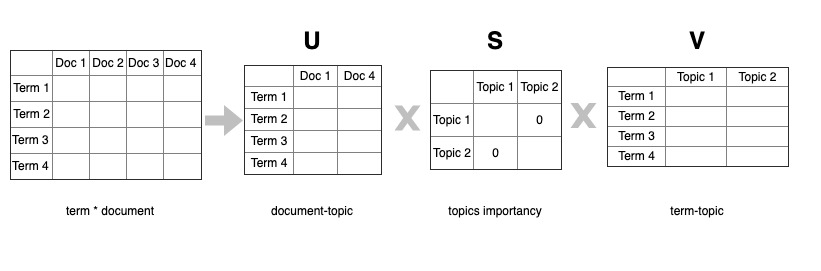
\includegraphics[width=1\textwidth]{diagrams/LSA.jpg}
\caption{
LSA matrix decomposition.}
\label{fig:svd}
\end{figure}
Selected $k$ greatest elements of $S$, corresponding columns from $U$ and rows from $V$ gives us k most important topics. $V$ than offers most important words for given topics.\par
LDA is based on the same assumptions. Unlike LSA, LDA assumes that topics and words follow Dirichlet's distribution. LDA tries to learn a model that best explains how data was generated.
\subsection{Implementation}
\label{sec:implementTM}
LDA model is created using package Gensim\footnote{\url{www.radimrehurek.com/genisim}} built by NLP Centre of the Masaryk University \cite{nlpcentre} especially for topic modeling, which pratically the only possible solution. We considered two libraries for NER task - \textit{NLTK}\footnote{\url{www.nltk.org}} and \textit{spaCy}. As using spaCy is much more comfortable than NLTK, we chose spaCy. Besides, SpaCy also seems to have superior performance on Twitter-like data \cite{TwitterNerComparison} (see Table \ref{tab:nerComparison}). These two considered libraries are not state-of-the-art possibilities, but provide reasonable results. The performance can be improved by using for example Standford CoreNLP, which is more technically demanding, but offers better precision. Socneto, though, expects human receiving result and than recall is maybe more importnant metric than precision, as mentioned also in \cite{TwitterNerComparison}. It is better to see all results and discard some wrongly classified than miss some results.

\begin{table}[h]
\footnotesize
%\begin{tabular}{@{}llll@{}}
\begin{tabular}{llll}
\textbf{System Name}                & \textbf{Precision}  & \textbf{Recall}   & \textbf{F1 Score}  \\
Stanford CoreNLP              & 0.526600541 & 0.453416149 & 0.487275761 \\
Stanford CoreNLP (with Twitter POS tagger) & 0.526600541 & 0.453416149 & 0.487275761 \\
TwitterNER                 & 0.661496966 & 0.380822981 & 0.483370288 \\
OSU NLP                  & 0.524096386 & 0.405279503 & 0.45709282 \\
Stanford CoreNLP (with caseless models)  & 0.547077922 & 0.392468944 & 0.457052441 \\
Stanford CoreNLP (with truecasing)     & 0.413084823 & 0.421583851 & 0.417291066 \\
MITIE                   & 0.322916667 & 0.457298137 & 0.378534704 \\
spaCy                   & 0.278140062 & 0.380822981 & 0.321481239 \\
Polyglot                  & 0.273080661 & 0.327251553 & 0.297722055 \\
NLTK                    & 0.149006623 & 0.331909938 & 0.205677171 \\ 
\end{tabular}
\caption{Comparison of available NER models for Twitter data. Data comes from Workshop on Noisy User-generated text \cite{wnut} 2016. \newline \textit{source: \cite{TwitterNerComparison}}}
\label{tab:nerComparison}
\end{table}

SpaCy, in addition, offers a built-in preprocessing pipeline, which we  used in both LDA and NER. Such a pipeline aims to transform the raw text into something more organized. In the case of spaCy, it contains a tokenizer, tagger, parser and named entity recognizer (see Figure \ref{fig:pipeline}), where:
\begin{itemize}
  \item Tokenizer: Breaks the full text into individual tokens.
\item Tagger: Tags each token with part-of-speech tag as noun, pronoun, adjective, punctuation etc. \cite{tags},
\item Parser: Creates syntactic tree, finds noun phrases.
\item Named Entity Recognizer (NER): Labels named entities.
\end{itemize}
\begin{figure}[H]
\centering
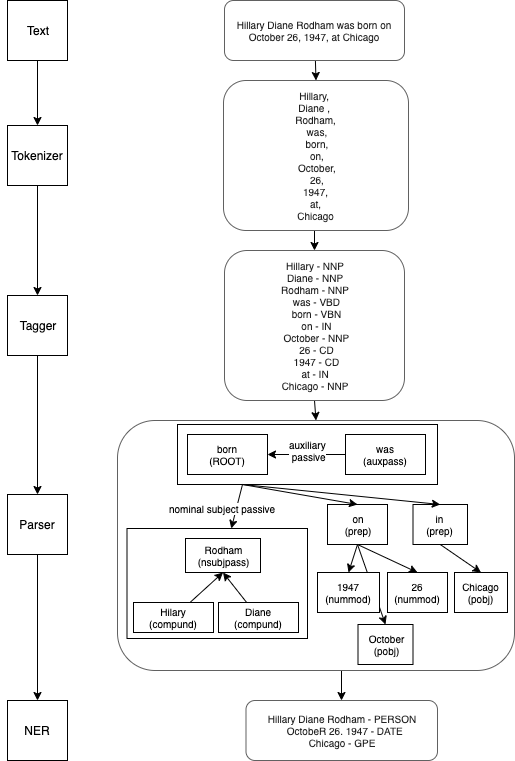
\includegraphics[width=0.7\textwidth]{diagrams/PIPELINE.png}
\caption{An example of processing in SpaCy pipeline.}
\label{fig:pipeline}
\end{figure}

\section{Sentiment Analysis (SA)}
\label{sec:sentiment}
We will consider the sentiment analysis task in the following form:
\begin{itemize}
    \item \textbf{Input:} A snippet of text (article, tweet etc.)
    \item \textbf{Output:} Classification into one of classes - positive, neutral, negative. 
\end{itemize}

Sometimes there is also considered so-called \textit{subjectivity} \cite{veselovska-2017}. It tries to classify if the opinion (both positive or negative) is objective or the author is personally interested and has strong emotions about his claims. For example, the following text could be recognized as objective: ``The sound of this notebook is clear.'', ``The base is not stable enough.'' or ``An internet connection in this area is bad.'' in contrast with ``I hate the way the new touchpad works.''. The subjectivity of the claim does not depend on its sentiment.
This part of sentiment analysis was not included in our project yet, but it is one of the possible extensions.
\subsection{Methods}
According to NLP-progress page \cite{sotasentiment}, actual state-of-the-art accuracy of this task on English datasets in the case of binary classification is above 95\%. Our demands, however, are higher than just binary classification. Classifying into more classes is noticeably harder, so our expectations about model performance are lower. As in the case of the TM task, some gold data labels could be subject to dispute, but it is still easier to classify into one of three given categories. \par
The chosen methods for this type of analysis are the Bidirectional Encoder Representations from Transformers (BERT) . The first idea of BERT was published in the first half of 2019 by Google AI Language \cite{bert} and since then, it is a leading approach to various NLP tasks. Not only that its results in many tasks are new state-of-the-art numbers, but its main advantage is a universality and easy use for different types of prediction. This allows distribution of non-specific pre-trained models, while fine tuning on any task could be done just by adding one simple layer on the top. This practice, known as \textit{transfer learning} has a long history in image processing. Unlike previous widely used models, BERT model just represents some universal knowledge about language. The next section is devoted to the further explanation of BERT ideas.
\subsection{BERT}
BERT model is built upon the idea of \textit{transformers}. A transformer is a neural network with two parts - encoder and decoder. Contrary to other types of neural networks, the input of a transformer is the whole sentence of text. Inputs are fed to the network in the form of embeddings, and the transformer tries to learn how to encode the sentence in the way that decoder can reproduce the original sentence. The whole training is an oscillation between decoder learning the best way to decode encoder output and encoder trying to learn better representation for the given sentence. In BERT, only the encoder is used. BERT model has three main features to describe - usage of embeddings, masked language modeling (MLM) and next sentence prediction. Each of them is described in the following text.
\subsubsection{Embeddings}
Following the transformers paper \cite{vaswani1706attention},
inputs are transformed into three types of embeddings: token embeddings, sentence embeddings and special transformer positional embeddings (see Figure \ref{fig:bert_emb}). These embeddings serve as a technical simplification for other model parts.

\begin{figure}[H]
\centering
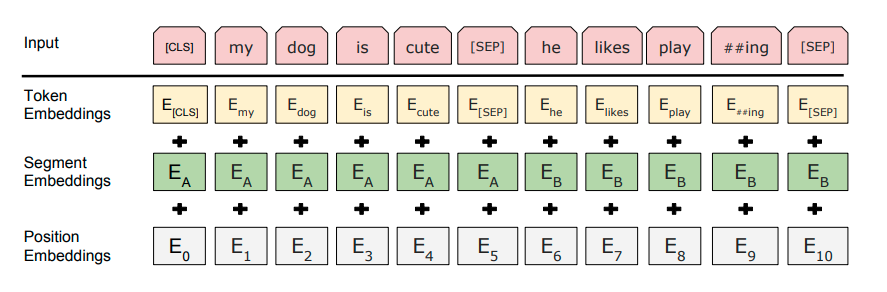
\includegraphics[width=1\textwidth]{diagrams/BERT-emb.png}
\caption{
Structure of BERT input embeddings. Input is enriched of tokens for start and end of sentences and then represented by embeddings for each word (token embeddings), embeddings for sentence (segment embeddings, same for words in one sentence) and position embeddings (position of token in the text).
\textit{source: \cite{bert}}}
\label{fig:bert_emb}
\end{figure}

\subsubsection{MLM}
MLM is a method for learning the language model. 15\% of input words are masked. Some of them will be visible at the end, but most of that, 12\%, is replaced by token [MASK].
This way the model improves the prediction of masked words based on the surrounding context.
\subsubsection{Next Sentence Prediction (NSP)}
NSP is a similar concept to MLM. In one part of the training, inputs of the model are pairs of sentences. In 50\% cases, the second sentence follows the first one in the training data. Otherwise, the second member of the pair is a random sentence from the data. The model then learns how to predict the following sentence.

\subsubsection{Whole Model}
MLM and NSP are combined and reflected in the loss function. The resulting language model is not trained to perform a specific task and this is done by stacking one or more layers at the top of this model. Then it is possible to combine training of these new layers only with allowing the gradient to flow through all model layers.

\subsection{Implementation}
The main third-party implementation to use for BERT is transformers by HuggingFace \cite{Wolf2019HuggingFacesTS}.
This library contains implementations of recent state-of-the-art ideas including BERT and its variations together with a pre-trained model on more than 100 languages. Pre-trained models are important because time demands on training the model from scratch even on school clusters \footnote{\url{https://gitlab.mff.cuni.cz/ksi/clusters}}. Orginal model was trained for four days on 4 to 16 Cloud TPUs. \footnote{\url{https://github.com/google-research/bert}}
 Transformers library provides prepared model architectures for tasks such as next sentence prediction, multiple-choice, classification, sequence classification or question answering. Transformers supports integration with tensorflow and keras packages. Tensorflow \cite{tensorflow2015-whitepaper} is an interface (and a package) dedicated to machine learning. Keras \cite{chollet2015keras} is a wrapper over tensorflow, which provides a shielding from too technical details. We could use Transformers method \textit{TfBertForClassification} for obtaining a model and then train it using Keras predefined method \textit{fit} or create own training loop using \textit{TensorFlow.GradientTape} construct. The first method requires padding all sentences to the same length, which could produce too long sentences and have a negative impact on running time. For the second method, padding sentences only to the length of maximum in one batch (as opposed to maximum over the whole dataset) is enough and there exists library \textit{\cite{Ktrain}}, a wrapper upon Keras, which can do it and is used in Socneto. \par
With a pre-trained model and working additional training, all that is needed is to fine-tune a model. Actually, there is more BERT-like models distributed in transformers library (and Ktrain too). Some of the differs from the original paper in later improvements and some of them are just larger. Socneto uses \textit{distilbert} model, which is small enough for a reasonable usage and offers good performance.
A comparison of results with different training parameters is offered in Section \ref{sec:Model_selection}. Here remains only to describe the training data. Although there exist many sentiment datasets, a large part of them is a binary classification (positive-negative) only. One of the three-classed datasets is Twitter US Airline Sentiment \cite{airlines}
containing almost 14,000 tweets about six American airlines. 70\% of them were used as training data, while 30\% served as validation data for verification of accuracy and detection of overfitting after every training episode. 
\subsection{Model Selection}
\label{sec:Model_selection}

Fine tuning is not just about creating a layer and putting training data in. There are always hyperparameters to set and the performance of models can vary a lot depending on them. In our case, the main hyperparameters to set are the learning rate, the number of episodes and the style of learning.
\subsubsection{Learning Rate}

The learning rate influences the speed of the learning by setting the size of one step through the space of the network weights. Too big learning rate can cause chaotic jumping here and there, which will never hit the optimum of the loss function. On the contrary,  too small learning rate is time inefficient and can also cause getting stuck in the saddle point. The Ktrain library allows usage of Keras method for searching the best learning rate. The output of this method is a plot of the learning rate versus the loss function. The best learning rate is around the point, where the loss function starts to decrease, which is around $10^{-6}$ in our case (see Figure \ref{fig:figlearningrate}).
\begin{figure}
\centering
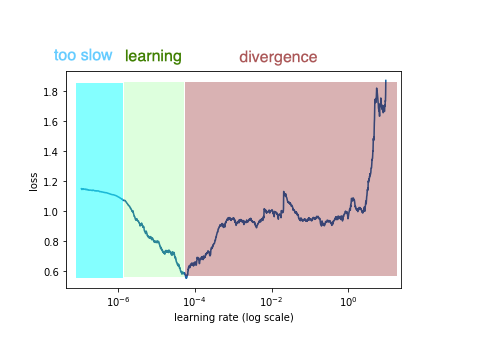
\includegraphics[width=0.8\textwidth]{diagrams/learning_rate2.png}
\caption{
Learning rate for \textit{distilbert} pre-trained model on airlines dataset.}
\label{fig:figlearningrate}
\end{figure}

\subsubsection{Training Strategy}
It is better to change the learning rate during training. In the beginning, when the model is bad, we want to find a better solution quickly. After some iteration, however, our model starts to be clever and it is unwanted to forget all and change the direction completely. Ktrain offers three possibilities of training - \textit{fit\_one\_cycle}, \textit{fit}, and \textit{autofit} (see Figure \ref{fig:strategies}).
\begin{figure}
\centering
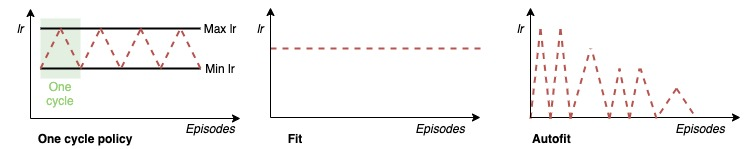
\includegraphics[width=1\textwidth]{diagrams/strategies.jpg}
\caption{
A comparison of different Ktrain training methods. On the left plot, learning rate is oscillating in every cycle between minimal and maximal learning rate. Cycle length can generally be different from epoch, but typically one cycle is one epoch long. The middle image shows just constant learning rate during whole training and the rightmost figure shows possibilities of autofit method to change learning rate after n periods without loss decrease (where n is a parameter).  
}
\label{fig:strategies}
\end{figure}
%TODO obrazek lepsi s porovnanim
 One cycle policy \cite{smith2018disciplined}goes from the lower bound to the upper bound in each cycle.
\textit{Autofit} method performs one cycle policy with cycle length equal to epoch for every epoch. It is also able to automatically decrease the learning rate if the loss on the validation set does not improve and stop training when it starts to diverge. The third method, \textit{fit}, is simple - it just uses the constant learning rate all the time.

\subsection{Experiments}
\label{sec:experiments}
In this section, different learning strategies effect is presented in a short overview. 
Experiments where performed for different learning rates and different strategies. 

Figure \ref{fig:acc_loss} plots progression of loss function and accuracy over 10 training epochs for tree different learning rates. For the \textit{fit} method, where constant learning rate is used, loss function starts to grow immediately after the first epoch, so further training just worsens results. One cycle policy for learning rates $4\cdot10^{-6}$ and $7\cdot10^{-6}$ is learning well for five or four epochs respectively, but best results are actually same or worse than one epoch with constant learning rate. Autofit starts to diverge, even when decrease of learning rate after 2 epochs with an increasing loss function was set for the greatest learning rate.

\begin{figure}[H]
\centering
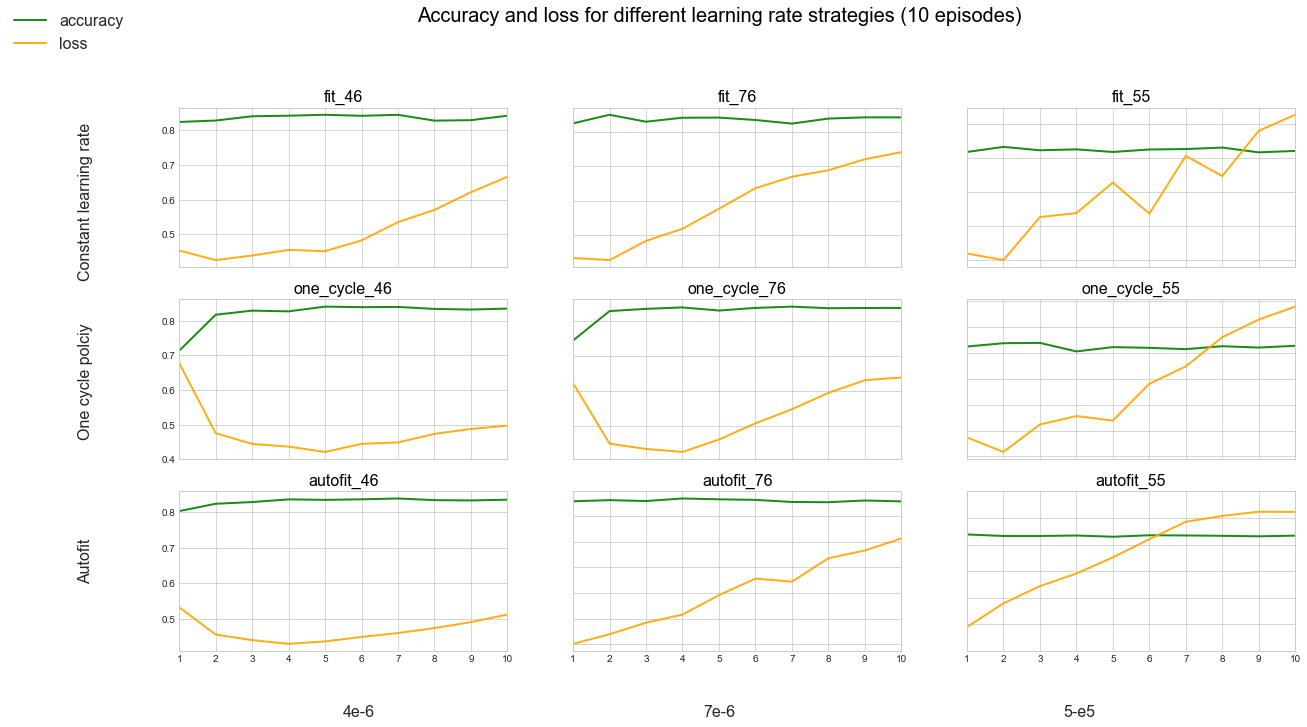
\includegraphics[width=1\textwidth]{diagrams/acc_loss.png}
\caption{ Loss and accuracy progress trough 10 training episodes.
}
\label{fig:acc_loss}
\end{figure}

There were performed other experiments using reduce of learning rate with different starting learning rate value. As starting on $8\cdot10^{-7}$ was slow, but with increasing learning rate over 20 episodes, starting with $6.25\cdot10^{-6}$ was to much and loss function grew for every episode. Neither of mentioned models was able to outperform the chosen one.


\par
For usage in Socneto, model \textit{fit\_76} from figure \ref{fig:acc_loss}, as it has the best accuracy. It is the model trained using only constant learning rate $7\cdot10^{-6}$ for 10 epoch. \\
\begin{center}
    

\begin{table}[H]
\label{table:resultsAnalysis}
\begin{tabular}{llll}
         & \textbf{precision} & \textbf{recall} & \textbf{f1 score} \\
\textbf{neutral}  & 0.87      & 0.82   & 0.84     \\
\textbf{positive} & 0.90      & 0.88   & 0.89     \\
\textbf{negative} & 0.94      & 0.87   & 0.96    
\end{tabular}
\caption{
Results for selected model for Socneto.}
\end{table}
\end{center}
As it is possible to see in table \ref{table:resultsAnalysis}, on the development data, the model is very good in recognizing negative texts (as the precision form negative is quite good) and the most hardly recognized are neutral posts.
